% ==========================================
% BÖLÜM 4.6: MOD_UI_VIEW (ARAYÜZ ÇİZİM VE RENDER KATMANI)
% ==========================================

\newpage
\section{\texttt{mod\_UI\_View}}

\texttt{mod\_UI\_View}, uygulamanın Grafik Kullanıcı Arayüzü (GUI) bileşenlerinin çalışma zamanında (\textit{Runtime}) dinamik olarak inşasından, görsel nesne parametrelerinin yapılandırılmasından ve hesaplanan verilerin ekran elemanlarına aktarılmasından (\textit{Rendering}) sorumlu Görünüm Katmanı (\textit{View Layer}) modülüdür.

Uygulamada standart \texttt{UserForm} yapısı yerine, \texttt{Worksheet} üzerine gömülen asenkron OLE Panelleri (\texttt{MSForms.Frame}) tercih edilmiştir. Bu mimari yaklaşımda \texttt{mod\_UI\_View}, arayüzün nesnel tasarım kalıplarına uygun şekilde soyutlanmasını sağlar. İş mantığı katmanı (\texttt{mod\_Services}) ile kullanıcı etkileşim katmanı (\texttt{mod\_UI\_Events}) arasında köprü kurarak, ham veriyi görsel tablolara (\texttt{ListBox}) dökme işlevini üstlenir.

Modülün temel tasarım ve mimari sorumlulukları üç ana grupta toplanmaktadır:

\begin{itemize}\setlength{\itemsep}{0pt}\setlength{\parskip}{1pt}
    \item \textbf{Dinamik Kontrol Oluşturma (UI Builder):} Çalışma sayfasına eklenecek \texttt{Frame}, \texttt{CommandButton}, \texttt{ListBox}, \texttt{Label}, \texttt{TextBox} ve \texttt{ComboBox} gibi nesnelerin koordinat, boyut, renk ve varsayılan durumlarını programatik olarak tanımlar.
    \item \textbf{Veri Bağlama ve Görselleştirme (Data Rendering):} Servis katmanından dönen dizileri ve koleksiyonları dinamik listelere yükler; hata durumlarında kullanıcıya durum göstergeleri (\texttt{OK}, \texttt{HATA}) sunar.
    \item \textbf{Olay Dinleyici Kaydı (Event Registration):} Çizilen her bir dinamik butonu, tıklama olaylarının yakalanabilmesi amacıyla merkezi \texttt{ButtonCollection} koleksiyonuna bağlar.
\end{itemize}

\vspace{0.15cm}

\begin{infobox}{\faPalette\ Arayüz Bileşenleri ve Modüler Yapı}
Görsel katmanda yer alan tüm panel oluşturma (\texttt{Create*}) ve veri işleme (\texttt{Render*}) Prosedürleri, \texttt{mod\_Config} modülündeki merkezi sabitleri (\texttt{PANEL\_WIDTH}, \texttt{COLOR\_GREEN} vb.) referans alır. Bu sayede arayüz tasarımındaki renk ve boyut değişiklikleri kod tekrarı olmadan tek bir noktadan yönetilebilir.
\end{infobox}

\vspace{0.3cm}

\textbf{\textcolor{primary}{1. Geliştirme Ortamı ve Modül Yapısı}}

Aşağıdaki ekran görüntüsünde, VBA Geliştirme Ortamı (\textit{VBE}) üzerinde \texttt{mod\_UI\_View} modülünün barındırdığı yapıcı, yardımcı ve render prosedürlerinin genel listesi sunulmaktadır:

\vspace{0.3cm}

\begin{figure}[htbp]
    \centering
    \fboxsep=0pt
    \fboxrule=0.8pt
    \fcolorbox{bordergray}{white}{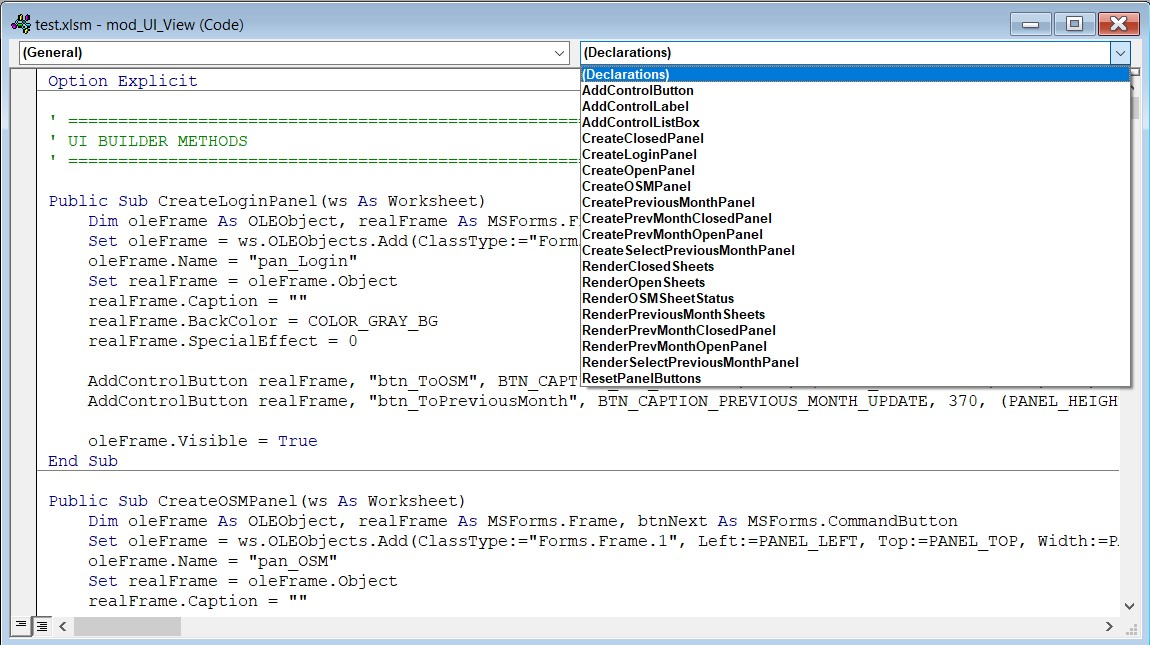
\includegraphics[width=0.88\textwidth, keepaspectratio]{mod_UI_View.jpg}}
    \caption{\texttt{mod\_UI\_View} Modülü Prosedür ve Fonksiyon Dizilimi}
    \label{fig:mod_ui_view_code}
\end{figure}

\vspace{0.2cm}

\textbf{\textcolor{primary}{2. Arayüz Oluşturucuları (UI Builder Methods)}}

Çalışma kitabı ilk açıldığında veya yapılandırma sıfırlandığında, sistemdeki her bir iş akışı paneli (\texttt{Login}, \texttt{OSM}, \texttt{Open}, \texttt{Closed}, \texttt{PreviousMonth}, \texttt{SelectPreviousMonth} vb.) özel oluşturucu prosedürler tarafından inşa edilir. 

Panel yapım aşamasında izlenen standart işlem adımları şunlardır:
\begin{enumerate}\setlength{\itemsep}{0pt}\setlength{\parskip}{1pt}
    \item Aktif sayfada \texttt{OLEObjects.Add} fonksiyonu ile yeni bir \texttt{MSForms.Frame} örneği açılır.
    \item Panelin arka plan rengi, kenarlık stili ve konum parametreleri ayarlanır.
    \item Yardımcı private metotlar (\texttt{AddControlButton}, \texttt{AddControlLabel}, \texttt{AddControlListBox}) kullanılarak panel içerisine gerekli kontrol elemanları yerleştirilir.
    \item Oluşturulan buton referansları bellek kaybolmasını önlemek için \texttt{clsDynamicButton} wrapper sınıfına tescil edilir.
\end{enumerate}

\vspace{0.3cm}

\textbf{\textcolor{primary}{3. Veri Render Yöneticileri (UI Renderer Methods)}}

Kullanıcı paneller arasında geçiş yaptığında veya tarama/güncelleme butonlarına bastığında \texttt{Render*} prosedürleri devreye girer. Bu prosedürler, arka plandaki servislerden dönen dinamik veriyi okur ve \texttt{ListBox} elemanlarını kolon genişliklerine göre biçimlendirerek doldurur.

\newpage
Render sürecinde öne çıkan temel mantıksal mekanizmalar:
\begin{itemize}\setlength{\itemsep}{0pt}\setlength{\parskip}{1pt}
    \item \textbf{Sütun Başlıkları ve Tablo Hizalama:} Her render işleminde \texttt{ListBox.Clear} ile liste sıfırlanır ve ilk satıra sabit tablo başlıkları yüklenir.
    \item \textbf{Otomatik Veri Dönüşümü ve Eşleme:} Veritabanı hücre adresleri (\texttt{D4}, \texttt{K2} vb.) ve ilişkili sayfa isimleri birleştirilerek açıklayıcı metinler (\textit{Örn: D4 (ARIZA)}) halinde listeye aktarılır.
    \item \textbf{Zamanlayıcı ve Otomatik Kilit Mekanizması:} Ekran render edildikten sonra tarama butonlarının aktif kalması ve hatalı çift tıklamaların önlenmesi amacıyla \texttt{Application.OnTime} kullanılarak panel belirli bir süre sonra otomatik kilit durumuna alınır.
    \item \textbf{Boş Satır Tamamlama (Dikey Izgara Düzeni):} Görsel bütünlüğü korumak amacıyla veriler yüklendikten sonra \texttt{ListBox} dikey boyutu dolana kadar boş satır tamamlama döngüsü (\texttt{Do While ListCount < 12}) çalıştırılır.
\end{itemize}

\vspace{0.15cm}

\begin{warningbox}{\faExclamationTriangle\ Arayüz Kararlılığı ve Hata İşleme}
Render işlemleri esnasında geçersiz sayfa yapıları veya silinmiş OLE nesneleri nedeniyle çökme yaşanmaması adına, buton sıfırlayıcı yardımcı prosedürlerde (\texttt{ResetPanelButtons}) yerel hata yönetimi (\texttt{On Error Resume Next}) uygulanmaktadır.
\end{warningbox}

\vspace{0.4cm}

\begin{tcolorbox}[colback=yellow!15,colframe=orange!80!black,leftrule=3.5pt,boxrule=0.4pt,top=5pt,bottom=5pt]
    \textbf{\textcolor{orange!80!black}{\faInfoCircle\ mod\_UI\_View Genel Özet ve Mimari Rolü:}}\\
    \small \texttt{mod\_UI\_View}, uygulamanın tüm görsel bileşenlerini ve tablo ekranlarını kod üzerinden dinamik üreten bir **Grafik Motoru** işlevi görür. Veri işleme mantığını görsel tasarımdan tamamen ayırarak (MVC mimari yaklaşımı), projenin sürdürülebilirliğine ve kolay genişletilebilir bir arayüz yapısına kavuşmasına doğrudan katkı sağlar.
\end{tcolorbox}